\subsection*{Solution to Fall 2010, \#1} \label{F10Q1}

First, observe that solutions to the homogeneous version of the differential equation are of the form $u_h(x) = a \sin(x) + b \cos (x)$ for constants $a$ and $b$.
To solve the non-homogeneous version of the equation, we guess that the particular solution is of the form $u_p (x) = cx + d$ for some constants $c$ and $d$.
Plugging $u_p$ into the differential equation yields $c=1$ and $d=A$. Hence, by the superposition principle, we have that the solution to the differential equation must be of the form
$$ u(x) = a \sin(x) + b \cos(x) + x + A $$
Enforcing the boundary conditions yields
$$ u(0) = b + A = 0 \quad \implies \quad b = -A $$
$$u(\pi) = -b + \pi + A = 0 \quad \implies \quad A = -\frac{\pi}{2} $$
Therefore, if $A = -\frac{\pi}{2}$, the solution to the differential equation is
$$ u(x) = a\sin(x) + \frac{\pi}{2} \cos(x) + x - \frac{\pi}{2} $$
for any constant $a$. \hfill \qed

\subsection*{Solution to Fall 2010, \#2}
\label{F10Q2}

\subsubsection*{Solution to $2a$}

The eigenvalues of $\smat{1}{4}{4}{1}$ are 5 and -3 with corresponding eigenvectors $\svt{1}{1}$ and $\svt{1}{-1}$. Thus,
$$ \pmat{1}{4}{4}{1} = \pmat{1}{1}{1}{-1} \pmat{5}{0}{0}{-3} \pmat{1/2}{1/2}{1/2}{-1/2} $$
Hence, we have
$$ \vct{u}{v}_t = \pmat{1}{1}{1}{-1} \pmat{5}{0}{0}{-3} \pmat{1/2}{1/2}{1/2}{-1/2} \vct{u}{v}_x $$
which can be rewritten as
$$\pmat{1/2}{1/2}{1/2}{-1/2} \vct{u}{v}_t = \pmat{5}{0}{0}{-3} \pmat{1/2}{1/2}{1/2}{-1/2} \vct{u}{v}_x$$
Let $\svt{y}{z} = \smat{1/2}{1/2}{1/2}{-1/2} \svt{u}{v}$. Then,
$$ \vct{y}{z}_t = \pmat{5}{0}{0}{-3} \vct{y}{z}_x $$
Furthermore, observe that
\begin{gather*}
y(x,0) = \frac{1}{2} u(x,0) + \frac{1}{2} v(x,0) = \frac{1}{2} (f(x) +g(x)) \\
z(x,0) = \frac{1}{2} u(x,0) - \frac{1}{2} v(x,0) = \frac{1}{2} (f(x) - g(x))
\end{gather*}
Because the equations are now decoupled from our change of coordinates, we only need to solve two transport equations. Thus, we have
\begin{gather*}
y(x,t) = \frac{1}{2} (f(x+5t) + g(x+5t)) \\
z(x,t) = \frac{1}{2} (f(x-3t) - g(x-3t))
\end{gather*}
Therefore,
$$ \vct{u}{v} = \pmat{1}{1}{1}{-1} \vct{y}{z} = \left(
\begin{array}{c}
\frac{1}{2} (f(x+5t) + g(x+5t)) + \frac{1}{2} (f(x-3t) - g(x-3t)) \\
\frac{1}{2} (f(x+5t) + g(x+5t)) - \frac{1}{2} (f(x-3t) - g(x-3t))
\end{array} \right) $$
\hfill \qed

\subsubsection*{Solution to $2b$}
We have
$$\pmat{1}{4}{4}{1} = \pmat{1}{1}{1}{-1}\pmat{5}{}{}{-3}\pmat{1}{1}{1}{-1}^{-1}.$$
Let $w = \svt{w_1}{w_2} = \smat{1}{1}{1}{-1}^{-1}\svt{u}{v}$. Since $\smat{1}{1}{1}{-1}$ is invertible,
wellposedness of the problem
$$\vct{u}{v}_{t} = \pmat{1}{4}{4}{1}\vct{u}{v}_{x}\quad \text{ in $x \geq 0, t \geq 0$}$$
with $u(x, 0) = f(x)$, $v(x, 0) = g(x)$, and $au(0, t) + bv(0, t) =0$ is equivalent to wellposedness of the problem
$$w_{t} = \pmat{5}{}{}{-3}w_{x}\quad \text{ in $x \geq 0, t \geq 0$}$$
with $w_{1}(x, 0) = \frac{1}{2}f(x) + \frac{1}{2}g(x)$, $w_{2}(x, 0) = \frac{1}{2}f(x)- \frac{1}{2}g(x)$,
and $cw_{1}(0, t) + dw_{2}(0, t) = 0$ where $c = a + b$, $d = a - b$.

The characteristics of $w_{t} = 5w_{x}$ are $x + 5t = x_0$ and the characteristics of $w_{t} = -3w_{x}$ are $x - 3t = x_0$.
\begin{center}
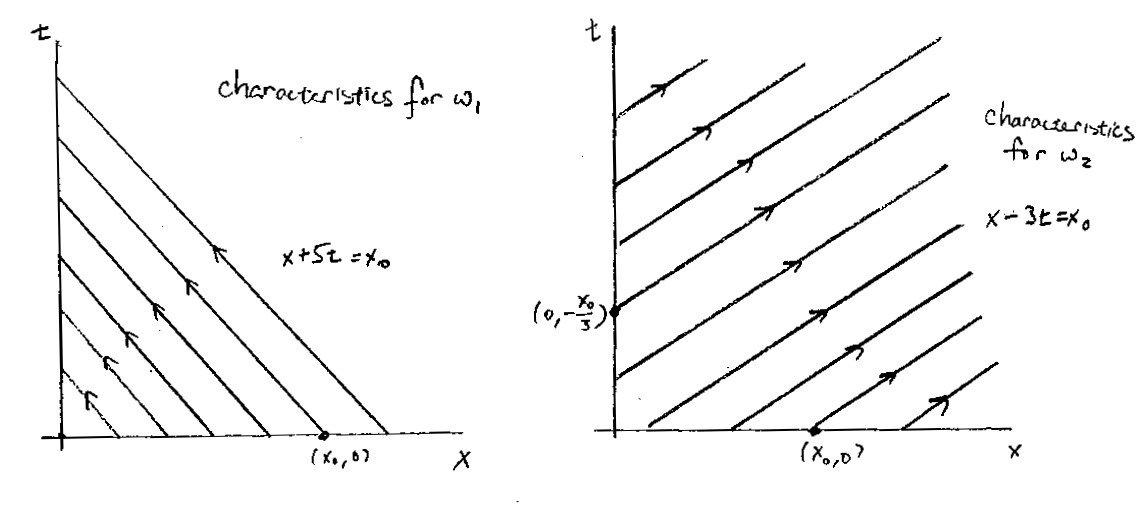
\includegraphics[scale=0.9]{./_Figures/F10Q2b.jpg}
\end{center}
Since $w_{1}$ is constant on characteristics,
\ba
w_{1}(x, t) = \frac{1}{2}f(x_0) + \frac{1}{2}g(x_0) = \frac{1}{2}f(x + 5t) + \frac{1}{2}g(x + 5t).
\ea
Then $w_{1}(0, t) = \frac{1}{2}f(5t) + \frac{1}{2}g(5t)$. As $cw_{1}(0, t) + dw_{2}(0, t) = 0$,
$$w_{2}(0, t) = -\frac{c}{2d}(f(5t) + g(5t)).$$
Since $w_{2}(x, 0) = \frac{1}{2}(f(x) - g(x))$,
\ba
w_{2}(x, t) &=
\begin{cases}
\frac{1}{2}(f(x - 3t) - g(x - 3t)) & \text{ if } x - 3t > 0\\
-\frac{c}{2d}(f(-\frac{5}{3}(x - 3t)) + g(-\frac{5}{3}(x - 3t))) & \text{ if } x - 3t < 0
\end{cases}\\
&=
\begin{cases}
\frac{1}{2}f(x - 3t) - \frac{1}{2}g(x - 3t) & \text{ if } x - 3t > 0\\
-\frac{c}{2d}f(5t - \frac{5}{3}x) - \frac{c}{2d}g(5t - \frac{5}{3}x) & \text{ if } x - 3t < 0.
\end{cases}
\ea
Thus the PDE is well posed as long as the boundary conditions for $w_{2}$ are compatible, that is,
we need $c$ and $d$ to be such that
$\lim_{t \rightarrow 0^{+}}w_{2}(0, t) = \lim_{x \rightarrow 0^{+}}w_{2}(x, 0)$.
That is,
$$-\frac{c}{2d}(f(0) + g(0)) = \frac{1}{2}(f(0) - g(0)).$$
Using that $c = a + b$, $d = a - b$, we have
$$\frac{a + b}{a - b} = \frac{g(0) - f(0)}{g(0) + f(0)}.$$
Rearranging yields
$af(0) = -bg(0)$.
Thus the set of $a, b$ which make the problem $\svt{u}{v}_{t} = \smat{1}{4}{4}{1}\svt{u}{v}_{x}$
with $u(x, 0) = f(x)$, $v(x, 0) = g(x)$, $au(0, t) + bv(0, t) = 0$ is precisely
the $a, b$ such that $af(0) = -bg(0)$.
\hq

\subsection*{Solution to Fall 2010, \#3}
\label{F10Q3}
\ssb{Solution to $(a)$}
The equilibria are $(0, 0)$, $(0, a_2/c_2)$, $(a_1/b_1, 0)$ and the solution to the system
$a_{1} = b_{1}x + c_{1}y$, $a_{2} = b_{2}x + c_{2}y$. Thus
$\svt{x}{y} = \smat{b_1}{c_1}{b_2}{c_{2}}^{-1}\svt{a_1}{a_2}$. Since $b_1 c_2 - b_2 c_1 \neq 0$, then
$\smat{b_1}{c_1}{b_2}{c_2}$ is invertible and hence the last equilibrium point is
\ba
\vct{x}{y} = \pmat{b_1}{c_1}{b_2}{c_{2}}^{-1}\vct{a_1}{a_2} = \frac{1}{b_1 c_2 - b_2 c_1}\pmat{c_2}{-c_1}{-b_2}{b_1}\vct{a_1}{a_2} = \frac{1}{b_1 c_2 - b_2 c_1}\vct{a_1 c_2 - a_2 c_1}{-a_1 b_2 + a_2 b_1}.
\ea
\hq

\ssb{Solution to $(b)$}
The equilibrium point in the open quarter plane is $(x_0, y_0)$ where
\ba
x_{0} = \frac{a_{1}c_{2} - a_{2}c_{1}}{b_{1}c_{2} - b_{2}c_{1}}, \quad y_{0} = \frac{a_{2}b_{1} - a_{1}b_{2}}{b_{1}c_{2} - b_{2}c_{1}}.
\ea
We will show that this point is a saddle. The Jacobian evaluated at $(x_{0}, y_{0})$ is
\ba
J(x_{0}, y_{0}) = \pmat{a_{1} - 2b_{1}x_{0} - c_{1}y_{0}}{-c_{1}x_{0}}{-b_{2}y_{0}}{a_{2} - b_{2}x_{0} - 2c_{2}y_{0}} = \pmat{-b_{1}x_{0}}{-c_{1}x_{0}}{-b_{2}y_{0}}{-c_{2}y_{0}}
\ea
where the last equality is because $a_{1} = b_{1}x_{0} + c_{1}y_{0}$ and $a_{2} = b_{2}x_{0} + c_{2}y_{0}$.
The eigenvalues of this matrix satisfy
\begin{align}\label{f103beq1}
\ld^2 + (c_{2}y_{0} + b_{1}x_{0})\ld + (b_{1}c_{2} - b_{2}c_{1})x_{0}y_{0} = 0.
\end{align}
Thus to prove the roots of \eqref{f103beq1} are distinct and real, it suffices to show that
$$(c_{2}y_{0} + b_{1}x_{0})^{2} - 4(b_{1}c_{2} - b_{2}c_{1})x_{0}y_{0} > 0.$$
We have
\ba
(c_{2}y_{0} + b_{1}x_{0})^2 - 4(b_{1}c_{2} - b_{2}c_{1})x_{0}y_{0} &= (c_{2}y_{0})^2 + (b_{1}x_{0})^2 - 2b_{1}c_{2}x_{0}y_{0} + 4b_{2}c_{1}x_{0}y_{0}\\
& = (c_{2}y_{0})^2 + (b_{1}x_{0})^2 + 2(b_{2}c_{1} - b_{1}c_{2})x_{0}y_{0} + 2b_{2}c_{!}x_{0}y_{0} > 0
\ea
since $b_{2}c_{1} - b_{1}c_{2} > 0$ and $b_{2}c_{1}x_{0} y_{0} > 0$. Thus $(x_{0}, y_{0})$ is a saddle.
\hq

\ssb{Solution to $(c)$}
%
%
%
% PICTURE
%
%
%
%

\subsection*{Solution to Fall 2010, \#4}
\label{F10Q4}

We use method of characteristics. Define $F(x,t,z,p,q) = q + zp + x = 0$, where $z := u$, $p := u_x$, and $q := u_t$. Then, we have
\begin{equation}
\label{f1041} \dot{t}(s) = 1, \quad t(0) = 0
\end{equation}
\begin{equation}
\label{f1042} \dot{x}(s) = z(s), \quad x(0) = x_0
\end{equation}
\begin{equation}
\label{f1043} \dot{z}(s) = -x(s), \quad z(0) = f(x_0)
\end{equation}
Solving \eqref{f1041} yields $t(s) = s$. Then combining \eqref{f1042} and \eqref{f1043} yields
\begin{equation}
\label{f1044}
\ddot{x}(s) + x(s) = 0, \quad x(0) = x_0, \,\,\, \dot{x}(0) = f(x_0)
\end{equation}
Solving \eqref{f1044} yields $x(s) = x_0 \cos(s) + f(x_0) \sin(s)$, and then plugging this back into \eqref{f1043} yields $z(s) = -x_0 \sin(s) + f(x_0) \cos(s)$. Thus, we have
$$ u(x,t) = -x_0 \sin(t) + f(x_0) \cos(t), \quad \text{where $x_0$ satisfies} \,\,\, x = x_0 \cos(t) + f(x_0) \sin(t) $$
If $f'(x) \geq 0$ for all $x$, we claim that the characteristics don't cross for $t \in (0,\pi/2)$. Indeed, if characteristics do cross, then, for $x_0 \neq x_1$,
$$ x_0 \cos(t) + f(x_0) \sin(t) = x_1 \cos(t) + f(x_1) \sin(t) $$
implies
$$ -\frac{\cos(t)}{\sin(t)} = \frac{f(x_1)-f(x_0)}{x_1 - x_0} \geq 0 $$
But $-\frac{\cos(t)}{\sin(t)} < 0$ for $t \in (0,\pi/2)$, which is a contradiction. Therefore, the solution will exist for $t \in [0,\pi/2)$. \hfill \qed


\subsection*{Solution to Fall 2010, \#5}
\label{F10Q5}
Note that as $\phi$ is smooth and 1-1, $u = 0$ on $\pr D$ if and only if $\wh{u} = 0$ on $\pr D$.
Let $v$ be smooth and of compact support. Then
\ba
\int_{D}-\sum_{i = 1}^{2}\pr_{x_{i}}(\beta(x)u_{x_{i}})v\, dx = \int_{D}fv\, dx.
\ea
We have
\ba
\int_{D}f(x)v(x)\,dx = \int_{\wh{D}}f(\phi^{-1}(y))v(\phi^{-1}(y))\wh{h}(y)\, dy = \int_{\wh{D}}\wh{f}\wh{v}\wh{h}\, dy
\ea
and
\ba
\int_{D}-\sum_{i =1}^{2}\pr_{x_i}(\beta(x)u_{x_i})v\, dx &= \int_{D}\sum_{i = 1}^{2}\beta(x)u_{x_i}v_{x_i}\, dx\\
& = \int_{\wh{D}}\sum_{i = 1}^{2}\beta(\phi^{-1}(y))u_{x_i}(\phi^{-1}(y))v_{x_{i}}(\phi^{-1}(y))\wh{h}(y)\, dy\\
& = \int_{\wh{D}}\wh{\beta}(y)\wh{h}(y)\sum_{i = 1}^{2}u_{x_i}(\phi^{-1}(y))v_{x_i}(\phi^{-1}(y))\, dy.
\ea
We have $y = \phi(x) = \svt{\phi_{1}(x)}{\phi_{2}(x)}$ and $\frac{\pr u}{\pr x_i} = \frac{\pr u}{\pr y_1}\frac{\pr y_1}{\pr x_i} + \frac{\pr u}{\pr y_2}\frac{\pr y_2}{\pr x_i}$.
Thus
\ba
u_{x_{i}}(\phi^{-1}(y)) = u_{y_i}(\phi^{-1}(y))(\phi_{1})_{x_i}(\phi^{-1}(y)) + u_{y_2}(\phi^{-1}(y))(\phi_2)_{x_i}(\phi^{-1}(y))
\ea
and we will write the right hand side as $\wh{u}_{y_1}\cdot (\phi_1)_{x_i} + \wh{u}_{y_2}\cdot (\phi_2)(x_i)$.
Thus
\ba
&\int_{\wh{D}}\wh{\beta}(y)\wh{h}(y)\sum_{i = 1}^{2}u_{x_i}(\phi^{-1}(y))v_{x_i}(\phi^{-1}(y))\, dy\\
& = \int_{\wh{D}}\wh{\beta}\wh{h}\sum_{i = 1}^{2}(\wh{u}_{y_1}(\phi_1)_{x_i} + \wh{u}_{y_2}(\phi_2)_{x_i})(\wh{v}_{y_1}(\phi_1)_{x_i} + \wh{v}_{y_2}(\phi_2)_{x_i})\, dy\\
& = \int_{\wh{D}}\wh{\beta}(y)\wh{h}(y) \sum_{i = 1}^{2}\bigg(\wh{u}_{y_{1}}(y)[(\phi_{1})_{x_{i}}(\phi^{-1}(y))]^{2} + \wh{u}_{y_{2}}(y)[(\phi_{1})_{x_{i}}(\phi^{-1}(y))][(\phi_{2})_{x_{i}}(\phi^{-1}(y))]\bigg)\wh{v}_{y_{1}}(y)\\
&\,\,\,\,\, + \bigg(\wh{u}_{y_{1}}(y)[(\phi_{1})_{x_{i}}(\phi^{-1}(y))][(\phi_{2})_{x_{i}}(\phi^{-1}(y))] + \wh{u}_{y_{2}}(y)[(\phi_{2})_{x_{i}}(\phi^{-1}(y))]^{2}\bigg)\wh{v}_{y_{2}}(y)\\
&= \int_{\wh{D}}\wh{\beta}(y)\wh{h}(y)\sum_{i = 1}^{2}M_{i}\vct{\wh{y_{1}}(y)}{\wh{u}_{y_{2}}(y)}\cdot \del \wh{v}\, dy
\ea
where
\ba
M_{i} = \pmat{[(\phi_1)_{x_i}(\phi^{-1}(y))]^{2}}{[(\phi_{1})_{x_i}(\phi^{-1}(y))][(\phi_2)_{x_i}(\phi^{-1}(y))]}{[(\phi_{1})_{x_i}(\phi^{-1}(y))][(\phi_2)_{x_i}(\phi^{-1}(y))]}{[(\phi_2)_{x_i}(\phi^{-1}(y))]^{2}}.
\ea
Since
\ba
\int_{\wh{D}}\vec{u}\cdot \del v\, dx = -\int_{\wh{D}}\del \cdot \vec{u} v\, dx,
\ea
we have
\ba
\int_{\wh{D}}\wh{\beta}(y)\wh{h}(y)\sum_{i = 1}^{2}M_{i}\vct{\wh{y_{1}}(y)}{\wh{u}_{y_{2}}(y)}\cdot \del \wh{v}\, dy = -\int_{\wh{D}}\del \cdot \bigg(\wh{h}(y)(\sum_{i = 1}^{2}\wh{\beta}(y)M_i)\vct{\wh{u}_{y_1}(y)}{\wh{u}_{y_{2}}(y)}\bigg)\wh{v}(y)\, dy.
\ea
Let $N := \wh{\beta}(y)(M_1 + M_2)$. Then
\ba
N\vct{\wh{u}_{y_{1}}}{\wh{u}_{y_{2}}} = \vct{N_{11}\wh{u}_{y_{1}} + N_{12}\wh{u}_{y_2}}{N_{21}\wh{u}_{y_{1}} + N_{22}\wh{u}_{y_{2}}}.
\ea
Thus
\ba
\del \cdot (\wh{h}(y)N\vct{\wh{u}_{y_{1}}}{\wh{u}_{y_{2}}}) = \sum_{j = 1}^{2}\frac{\pr}{\pr y_{j}}(\wh{h}(y)\sum_{k = 1}^{2}N_{jk}(y)\wh{u}_{y_k}(y)).
\ea
Therefore we have
\ba
-\int_{\wh{D}}\sum_{i = 1}^{2}\frac{\pr}{\pr y_{i}}(\wh{h}(y)\sum_{j =1}^{2}N_{ij}(y)\frac{\pr\wh{u}}{\pr y_j}(y))\wh{v}(y)\, dy = \int_{\wh{D}}\wh{f}(y)\wh{h}(y)\wh{v}(y)\, dy
\ea
which proves the desired result.
\hq



\subsection*{Solution to Fall 2010, \#6}
\label{F10Q6}

\subsubsection*{Solution to $6a$}

Suppose $a > 1$, and define $V = \sq{u \in H^1(\Omega) \, : \, \frac{\partial u}{\partial n} = 0}$. Because of the homogeneous Neumann boundary condition, it's easy to verify that the (positive) Laplacian operator is a symmetric elliptic operator. (Note: symmetric in this sense means that the associated bilinear form satisfies $B[u,v] = B[v,u]$ for all $u,v \in V$.) This implies that there exists an orthogonal basis of eigenfunctions $\{\varphi_n\}_{n \in \N}$ associated with the eigenvalues $\{\lambda_n\}_{n \in \N}$. Note that 0 is an eigenvalue since all constant functions are associated eigenfunctions. Without loss of generality, let $\lambda_1 = 0$ and $\varphi_1(x) = 1/|\Omega^a|^{1/2}$, where $|\Omega^a|$ two-dimensional area of $\Omega^a$. From this, we suppose our solution has the form
$$ u(x) = \sum_{n=1}^{\infty} \alpha_n \varphi_n(x) $$
for some sequence $\{\alpha_n\}_{n \in \N}$. Because $\{\varphi_n\}_{n \in \N}$ is an orthogonal basis of eigenfunctions, we have
$$ f(x) = \sum_{n=1}^{\infty} f_n \varphi_n(x), \quad \text{where} \,\,\, f_n = \frac{\int_{\Omega^a} f(x) \varphi_n(x) \, dx}{\int_{\Omega^a} \varphi_n^2(x) \, dx} $$
Then, for $n \geq 2$,
$$ \Delta u = f \quad \implies \quad \lambda_n \alpha_n = f_n \quad \implies \quad \alpha_n = \frac{f_n}{\lambda_n} $$
Observe
$$ \Delta \varphi_1 = 0, \quad \text{and} \quad f_1 = \frac{1}{|\Omega^a|^{1/2}} \int_{\Omega^a} f(x) \, dx = 0 $$
so we may choose $\alpha_1=0$. Hence,
$$ u(x) = \sum_{n=2}^{\infty} \frac{f_n}{\lambda_n} \varphi_n(x) $$
Therefore, for $a>1$, a solution exists.

Now, suppose $0<a<1$. This implies that $\Omega^a$ is now disconnected. Suppose there exists a solution $u$ to the Neumann problem in this case. Then,
\begin{align*}
\int_{\Omega_+^a} \Delta u \, dx = \int_{\Omega_+^a} f \, dx \quad \implies \quad 0 = 1	
\end{align*}
which is a contradiction. Integration by parts was applied to the integral on the left, and the integral over the boundary vanishes because of the homogeneous Neumann boundary condition on $u$. Hence, no solution exists when $0<a<1$.

\subsubsection*{Solution to $6b$}

Fix $a>1$, and let $L^a = \partial \Omega_+^a \cap \Omega_-^a$. Then,
$$ 1 = \int_{\Omega_+^a} f \, dx = \int_{\Omega_+^a} \Delta u \, dx = \int_{\partial \Omega_+^a} \frac{\partial u}{\partial n} \, dx = \int_{L^a} \frac{\partial u}{\partial n} \, dx $$
Hence,
$$ 1 \leq |L^a| \sup_{L^a} \left| \frac{\partial u}{\partial n} \right| \leq |L^a| \sup_{\Omega^a} |\nabla u| $$
where $|L^a|$ is the length of $L^a$. We obtain the second inequality because $L^a \subset \Omega^a$. Then,
$$ \frac{1}{|L^a|} \leq \sup_{\Omega^a} |\nabla u| $$
Decreasing $a$ to $1$ means $|L^a| \to 0$, which yields
$$\sup_{\Omega^a} |\nabla u| \to \infty$$ \hfill \qed


\subsection*{Solution to Fall 2010, \#7}
\label{F10Q7}

Define $y(x,t) := u(x,t) - w(x)$, and observe
\begin{equation}
\label{f107heat}
	y_t - \Delta y = u_t - \Delta u + \Delta w = 0
\end{equation}
with $y(x,t) = 0$ on $\partial D$ and $y(x,0) = -w(x)$. Now, suppose $y(x,t) = F(x)G(t)$ for some functions $F$ and $G$. Plugging this into \eqref{f107heat} yields
$$ F(x) G'(t) - \Delta F(x) G(t) = 0 \quad \implies \quad \frac{G'(t)}{G(t)} = \frac{ \Delta F(x)}{F(x)} = -\mu $$
where $\mu$ is an arbitrary constant. This provides us with an ODE for $x$:
\begin{equation}
\label{f107eq1}
-\Delta F(x) = \mu F(x), \quad F = 0 \,\, \text{on} \,\, \partial D
\end{equation}	
We also have an ODE for $t$, but we aren't going to worry about it until after we solve \eqref{f107eq1}. Note that \eqref{f107eq1} is an eigenvalue problem for the (negative) Laplacian operator with homogeneous boundary conditions. It's straightforward to see that the operator is a symmetric elliptic operator, implying that there exists an orthogonal basis of eigenfunctions $\{\varphi_n\}_{n \in \N}$ with associated eigenvalues $\{ \lambda_n \}_{n \in \N}$. It's also easy to verify that $\lambda_n > 0$ for all $n \in \N$. From this, for each $n \in \N$, we obtain an ODE for $t$:
$$ G_n'(t) = -\lambda_n G_n(t) $$
(Note, by the superposition principle, we are now supposing that our solution takes the form $y(x,t) = \sum_{n=1}^{\infty} G_n(t) \varphi_n(x)$.) To obtain the initial conditions for this family of ODEs, we need to first represent $y(x,0) = -w(x)$ in terms of the eigenfunctions:
$$ -w(x) = \sum_{n=1}^{\infty} \alpha_n \varphi_n(x), \quad \text{where} \,\,\, \alpha_n = \frac{-\int_D w(x) \varphi_n(x) \, dx}{\int_D \varphi_n^2(x) \, dx} $$
Hence, for each $n \in \N$, we have
$$ G'_n(t) = -\lambda_n G_n(t), \quad G_n(0) = \alpha_n \quad \implies \quad G_n(t) = \alpha_n e^{-\lambda_n t} $$
Putting everything together yields
$$ y(x,t) = \sum_{n=1}^{\infty} \alpha_n e^{-\lambda_n t} \varphi_n(x) $$
Therefore,
$$ u(x,t) = w(x) + \sum_{n=1}^{\infty} \alpha_n e^{-\lambda_n t} \varphi_n(x) $$
Furthermore, there is no leading term in the asymptotic expansion of $u(x,t) - w(x)$ as $t \to \infty$ because $\lambda_n > 0$ for all $n \in \N$ --- all of the terms vanish in the limit. \hfill \qed



\subsection*{Solution to Fall 2010, \#8}
\label{F10Q8}

Let $E(t) := \frac{1}{2} \int_D u_t^2 + |\nabla u|^2 \, dx$. Then, differentiating with respect to $t$ and applying integration by parts yields
$$ \dot{E}(t) = \int_D u_t u_{tt} + \nabla u \cdot \nabla u_t \, dx = \int_D u_t u_{tt} - \Delta u u_t \, dx $$
Because $u$ vanishes on the boundary, the boundary integral that arises from integration by parts vanishes. Thus,
$$ \dot{E}(t) = - \int_D (a(x,t)u_t)^2 \, dx \leq 0 $$
Since $E(0) = \frac{1}{2} \int_D g(x)^2 + |\nabla f(x)|^2 \, dx < \infty $, we have
$$ 0 \leq E(t) \leq E(0) $$
for all $t$. Since $u=0$ on $\partial D$, by Poincare's inequality,
$$ \int_D u^2 \, dx \leq C_D \int_D |\nabla u|^2 \, dx \leq 2C_D E(t) \leq 2C_D E(0) $$
where $C_D$ is a constant that only depends on $D$. Therefore, $\int_D u^2 \, dx$ is bounded. \hfill \qed
